\chapter{绪论}
CFD数值模拟在航空航天飞行器气动优化设计等应用中发挥着重要作用,
但是全阶CFD模拟经济、时间成本高昂,限制了设计人员进行全面、快速的设计空间探索和设计迭代。为了以更省时省力、又快又好地获得最优解,机器学习等智能算法和技术在气动优化的寻优算法及构建代理模型、降阶模型等方面有广泛的应用,但是传统机器学习方法适用于处理低维数据,难以推广到复杂的CFD应用场景。随着人工智能领域的快速发展,以深度学习为代表的智能方法和技术在处理高维复杂数据上展现了强大的学习能力,从而为快速、精确气动评估提供了新思路和新方法。



\section{研究背景及意义}
计算流体力学( Computational Fluid Dynamics,简称 CFD )作为了解和探索流体运动的手段,在航空航天,交通运输,石油勘探,天气预测,水利工程和石油化工等工程领域发挥着极其重要的作用。近年来,随着计算机性能的提升,CFD的应用前景进一步扩大,渗透到生活的方方面面。小到吸管设计,大到汽车制造,生活中随处可见CFD的身影。在2020年新冠疫情期间,CFD研究者通过对喷嚏飞沫的流动状态进行研究,得出喷嚏飞沫可以漂浮8米远的结论,为疫情防控做出了重要的贡献\cite{JAMA-喷嚏}。

复杂飞行器气动优化设计是CFD的重要应用领域,以增升减阻为目标的气动优化是飞行器设计的重要组成部分。
如文献\cite{增升减阻ep}指出,对于某民航客机,起飞升阻比每提高1\%,可增加14个乘客;
着陆最大升力系数每增加1\%,则可增加22个乘客。
由此可见,提升气动优化效率,实现快速、精准的气动评估对于推动飞行器设计发展具有重要意义。
尽管传统的全阶CFD数值模拟可针对特定状态获得较高精度的评估结果,但是时间、经济等成本巨大。
为了以更省时省力、又快又好地获得最优解,许多研究者在优化设计时对原始模型进行简化处理,包括采用更为简单的代理模型\cite{代理模型}和降阶模型\cite{降阶模型},代替复杂的CFD评估过程,减少计算开销;引入基于机器学习的智能方法和技术等。因此,在保证模拟精度的基础上,不断地提升气动模拟的效率是数值模拟领域现阶段的研究热点,具有极大的实际应用价值。然而加速和优化气动评估目前面临着以下挑战:

\vspace{-0.2cm}
\begin{itemize}
	\item[(1)] 气动优化往往涉及许多相互交织影响的因素。以常见的超临界机翼优化为例,除需考虑巡航升阻力系数、升阻比、力矩系数等设
	计点性能外,抖振、阻力发散等非设计点动态特性也需考虑;同时,优化还存在一些必要约束,如机翼厚度、油箱容积、前后缘装置等。海量设计参数容易导致设计空间“爆炸”,仅依靠传统的CFD数值模拟极大地限制了对复杂飞行器进行全面的设计空间探索。
	\item[(2)] 机器学习等智能算法和技术,通过部分或者全部代替复杂的CFD评估过程,在原始模型简化处理方面有广泛的应用。
	然而,大部分机器学习技术借助于发展成熟的机器学习方法和技术,属于浅层学习方法,随着CFD所模拟的问题越加的复杂,其预测精度和应用范围相对有限。
	此外,传统机器学习算法复杂度将随着样本数量和模
	型精度的提高呈指数级增长,目前应用范围多限于一些容易获得训练样本的二维简单优化
	问题。

\end{itemize}

自2006年Hinton等提出深度信念网络\cite{深度信念网络}以来,在GPU、TPU等高性能计算机硬件的助力下,
以深度学习为代表的智能方法和技术迅速发展,成功应用于图像分类与识别,医疗诊断,视频预测,自然语言处理等诸多领域。
在学术界,深度学习算法和技术包括其相关应用也是世界各大研究实验室和顶尖大学的研究热点,
比如斯坦福大学、纽约大学、加拿大蒙特利尔大学等成为研究深度学习的重镇,在国际顶尖会议和期刊上涌现了许多关于深度学习的研究内容;
在工业界,包括众多互联网公司在内的知名企业专门设立了深度学习实验室,促进深度学习技术转化落地。

由于采用了复杂和更深层次的模型结构,深度学习模型更善于从数据中提取特征,而不是依靠人工构建特征,极大提升了归纳能力,
能够自主进行特征选择,可以从大量的候选特征中剔除无用特征再进行回归和分类,具备
深层次学习能力,尤其适合于归纳、分析高维、时空相关的流场数据,展现出广阔的应用前景。

一方面,深度学习方法拥有巨大的潜力解决CFD领域所面临的问题;另一方面,
基于深度学习的气动评估及其在气动优化中的应用尚处于起步阶段,已有应用多为二
维简单外形算例,多参考深度学习在其他领域应用较为成熟的方法技术,尤其是深度卷积
神经网络在计算机视觉领域的研究成果,深度学习还没有与空气动力学实现交叉融合。
因此,研究基于深度学习的气动优化技术对于解决气动优化领域所面临的问题和满足设计空间探索的实际需求具有重大意义。



\section{研究现状}
如图\ref{fig:1}所示,早在20世纪70年代就出现气动优化的应用,相关研究主要聚焦于使用小扰动方程、全势流等快速方
法进行气动评估\cite{70年代1,70年代2},结合梯度类优化算法对气动性能进行优化。
在20世纪80年代,以遗传算法为代表的进化类算法和以蚁群算法与模拟退火为代表的启发式算法
逐渐得到应用\cite{2000Aerodynamic,Genetic,Obayashi1995Genetic},这类方法不需要引入梯度信息,因其优化过程具有随机性,使用者无需关心优化的细节,所以在当时被广泛应用到气动优化过程。
但是,进化类算法依赖大量适应度函数分析,优化效率较低。
伴随方法\cite{Jameson2000Aerodynamic}的提出再次推动了基于梯度的优化方法的发展,通过求解伴随场,有效提升了求解梯度的效率。
为了结合两类算法的优点,混合算法在2000年以后开始得到广泛应用,实现局部寻优和全局寻优能力的均衡,通过将优化分阶段提高搜索效率等。

\begin{figure}[htp]
	\centering
	%\includegraphics[width=0.42\textwidth]{data/MLP.pdf}
	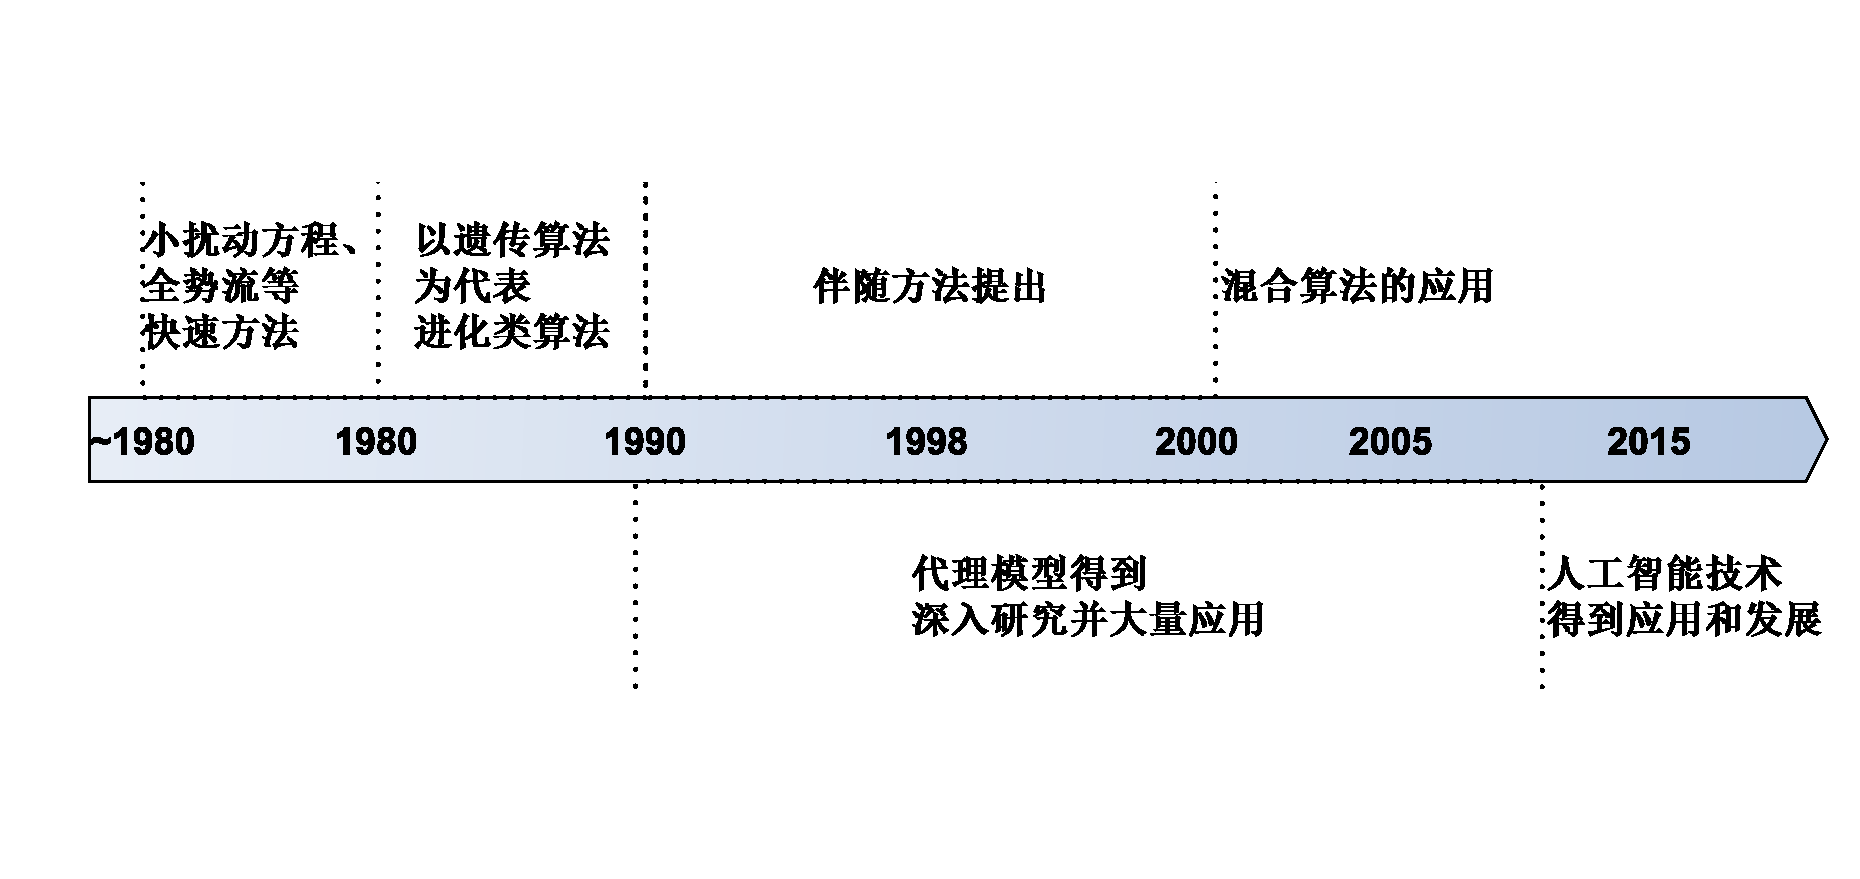
\includegraphics[width=0.92\textwidth]{figures/develop.pdf}
	\caption{气动优化技术的发展历程}
	\label{fig:1}
\end{figure}

随着机器学习技术和人工神经网络的发展,许多学者对以智能学习为基础的气动流场和气动性能预测方法进行了大量研究,基于智能学习的气动优化也是领域研究热点和本文关注的重点。
通过总结相关文献,本文对基于智能学习的气动优化技术和研究进行了整理和分类。
如图\ref{fig:智能优化}所示,基于智能学习的气动优化技术概括而言主要有两种:
一是利用传统机器学习方法和技术构建优化器、代理模型、降阶模型来减少计算开销,采用数据驱动方式,
通过对大量训练样例的“学习”构建数据间内部关系的模型,对未知数据进行预测;
二是基于深度学习方法和技术对气动特性和气动性能进行预测,利用深度神经网络强大的归纳学习能力,
提取高维、时空相关流场数据中的重要信息,构建气动流场、气动性能快速预测模型。

\begin{figure}[htp]
	\centering
	%\includegraphics[width=0.42\textwidth]{data/MLP.pdf}
	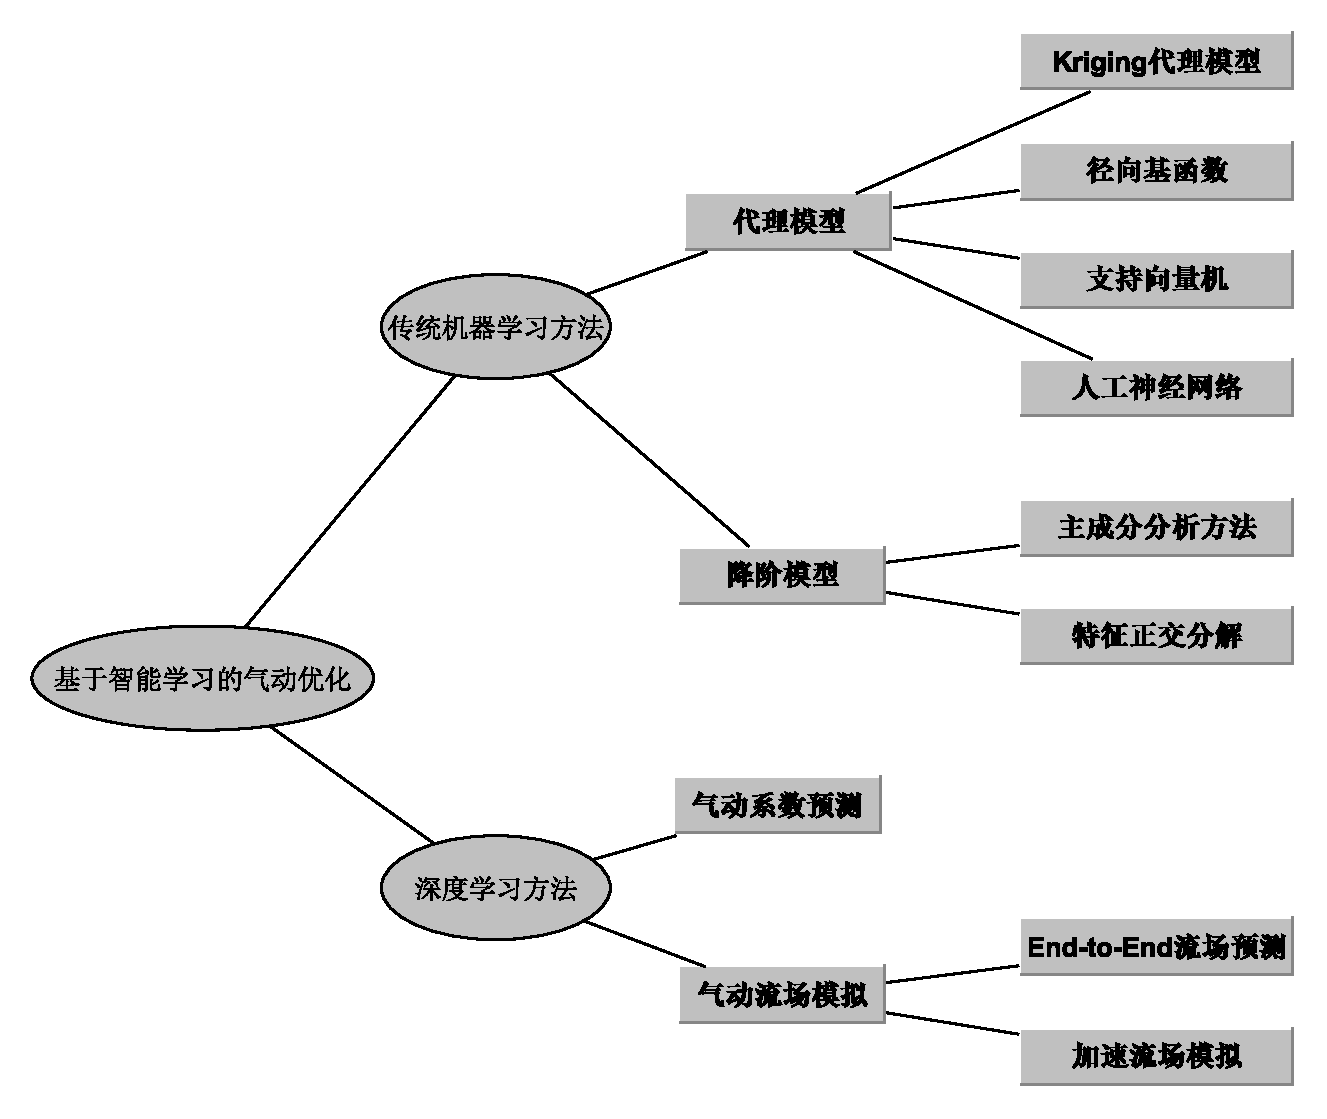
\includegraphics[width=0.92\textwidth]{figures/aicfd.pdf}
	\caption{基于智能学习的气动优化技术}
	\label{fig:智能优化}
\end{figure}

\subsection{基于传统机器学习的气动优化}
传统机器学习方法在气动优化中最典型的应用就是基于响应面法(response surface methodology,RSM)、多项式回归函数(Polynomial Regression,PR)、径向基函数(Radial Basis Functions,RBF)和人工神经网络(Artificial Neural Networks,ANN)等方法构建模型,快速从已计算的样本中预测设定的目标函数,从而达到代替CFD数值模拟的效果。此类优化方法通常被称为基于代理模型的优化方法。

Kanazaki和Tanaka等人\cite{Kanazaki2007Multi}针对飞机降落和接近失速条件下机翼升力系统的设计和优化问题,首先利用基于雷诺平均Navier-Stokes的CFD方法获取训练样本,设计了基于克里格(Kriging)代理模型的最大化升力系数的目标函数,实验结果表明相对于传统的遗传算法克里格模型显著降低了计算开销,同时实现了更好的性能。此外,作者还利用数据挖掘中的方差泛函分析方法分析了影响升力系统设计的主要因素。

张彬乾和罗烈等人\cite{张罗}针对飞翼布局设计中气动与隐身设计矛盾更为突出的问题,采用高精度气动和隐身计算方法,利用RBF神经网络代替复杂目标函数的评估,结合遗传算法和松散式代理模型管理方法,建立了翼型多目标优化设计平台。实验结果证明基于RBF神经网络的代理模型能有效模拟和评估翼型等几何形状与气动和隐身特性之间存在的强烈非线性关系。

Ju和Zhang等人\cite{Ame}为了解决蒙特卡罗模拟方法耗时长、计算开销大的问题,深入比较了人工神经网络、径向基函数和支持向量机模型(Support Vector Machine,SVM)的拟合精度,结果表明SVM精度较高,并以此基于SVM、遗传算法和蒙特卡罗方法针对翼型表面粗糙度的不确定性对翼型升阻系数进行了鲁棒性优化,实验结果表明,遗传算法-支持向量回归模型可以很好地捕获从表面粗糙度到机翼气动性能的不确定性传播。

基于代理模型的方法主要关注在给定输入数据的条件下,模型预测结果的准确性。
当研究输入变量之间的关系或者代理模型难以处理高维数据时,往往需要借助以主成分分析( Principal Component Analysis,PCA )和特征向量分解( Poper Orthogonal Decomposition,POD )为代表的机器学习方法。
比如,Kapsoulis和Dimitrios等人\cite{Kapsoulis2018Evolutionary}针对气动优化中维数灾难问题,整合进遗传算法和PCA方法,
在交叉和变异阶段使用PCA对设计变量进行降维,在降低优化复杂度的同时促使新个体的变化方向
沿着方差最大的方向进行,以提高优化效率。
此外,PCA和POD还可以用来对偏微分方程组进行降阶,得到降阶模型,再结合基于代理模型的方法,直接对气动流场进行预测。

\subsection{基于深度学习的气动优化}
近年来,以深度学习为代表的人工智能技术取得了令人瞩目的发展和成就,
深度学习等智能方法、技术也为快速、精确气动评估提供了新手段。
根据气动优化的目标不同,可以将基于深度学习的气动优化技术分为气动系数预测技术和气动流场模拟技术。
气动系数预测技术利用深度神经网络对感兴趣的气动系数(比如飞行器升力系数,升阻比等)进行回归预测,不关心流体在流场中运动的细节,属于深度学习在气动优化中的浅层运用。

Zhang和Sun等人\cite{LiftCoefficient}探讨了卷积神经网络技术的适应性以实现空气动力学元建模任务。
针对可变的流动条件和物体的几何形状,即具有多种形状的翼型,具有多个流动马赫数,雷诺数和攻角的流动条件,
训练了多个卷积神经网络以预测机翼的升力系数。
证明利用深度学习对空气动力学任务进行元建模的有效性。
将卷积神经网络结果与多层感知机的结果进行比较,发现基于卷积神经网络的元建模方法与多层感知机在学习能力方面具有可比性;
更重要的是,在几何表示约束最小的条件下,卷积神经网络模型预测准确性更高。

陈海和钱炜祺等人\cite{陈海2018}提出了一种基于深度学习的翼型气动系数预测方法,有效克服了以往方法依赖翼型设计参数以及算法复杂度随预测精度的提高呈指数级增长等缺点。该方法能够在只给出翼型图像的基础上,使用深度卷积神经网络根据翼型图像对其气动力系数进行了建模。研究结果表明显示模型预测的翼型气动系数获得了较高的精度,说明深度学习在翼型气动系数预测方面具有很好的应用前景。

利用深度学习技术对气动流场进行模拟,研究者可以观察到物理量(比如速度和压力)在流场中的分布,
获取更多有用的信息,对飞行器设计等工作进行针对性的优化和调整。
本文进一步对基于深度学习的流场模拟进行了分类:基于深度学习的流场预测方法和基于深度学习的流场模拟加速方法。
前者使用深度学习技术全部取代CFD过程实现End-to-End(端到端)流场预测,后者将深度学习方法作为加速模块并与传统的CFD求解器进行融合。

在基于深度学习的流场预测方法中,除了在神经网络模型训练阶段,需要利用CFD求解器准备训练数据以外,在模型训练完成后,推理过程不再依赖CFD方法,深度学习模型可以独立地对给定的几何体和流场条件进行预测。近年来,在基于深度学习的流场预测方向涌现了大量工作。

惠心雨和袁泽龙等人\cite{惠心雨2019}为了克服传统CFD计算需要耗费大量的计算时间与成本的缺陷,提出了一种基于深度学习的非定常周期性流场的预测框架,可以实时生成给定状态的高可信度的流场结果。将条件生成对抗网络(Generative Adversarial Networks,GAN)与卷积神经网络相结合,改进条件生成对抗网络对生成样本的约束方法,建立了基于深度学习策略采用改进的回归生成对抗网络模型,并与常规的条件生成对抗网络模型的预测结果进行对比。研究表明,基于改进的回归生成对抗网络的深度学习策略能准确预测出指定时刻的流场变量,且总时长比CFD数值模拟减少至少1个量级。

Guo和Li等人\cite{DBLP:conf/kdd/GuoLI16}针对非一致稳态层流流动建立了基于卷积神经网络(Convolutional Neural Network,CNN)的预测模型,其深度网络架构中包含了卷积编码和卷积解码(Encoder-Decoder)两部分,采用基于笛卡尔网格计算得到的符号距离函数(Signed Distance Function,SDF)作为输入,以LBM(Lattice Boltzmann Methods)求解器的模拟结果(速度场)作为训练样本标签。相对于基于二进制的几何外形表示,SDF值不仅提供了局部几何外形细节,同时包含了全局几何结构的丰富信息。作者针对二维简单形状、包含三维球体和圆柱的管道流等算例速度场进行了训练和预测,获得了较高的精度。深度神经网络预测耗时较GPU平台上LBM模拟快了2个数量级,较CPU平台上LBM模拟则快了4个数量级。该方法可以在早期设计阶段设计迭代中提供快速反馈,为构建实时、交互式设计优化空间探索提供了可能。

在Guo和Li等人的研究基础上,Bhatnagar和Afshar等人\cite{bhatnagar2019prediction}进行了改进,采用类似的深度神经网络架构,以3个翼型、4个雷诺数、21个攻角构成的RANS模拟结果作为训练数据,预测未知翼型、雷诺数、攻角的测试算例的速度场和压力场。与Guo等人的研究不同的是,作者在训练输入中增加了雷诺数、攻角信息( 在深度神经网络的全连接层处输入),且在损失函数中引入了gradient sharpening和L1正则化,提高了模型泛化能力和预测精度。

Miyanawala和Jaiman\cite{2017An}使用CNN预测了不同的阻流体的低雷诺数下的阻流体的空气动力系数。 他们提出了一种使用CNN和随机梯度下降法的数据驱动方法,用于在非定常流动问题中对Navier-Stokes方程进行模型简化。

Lee和You等人\cite{lee2019data}使用深度学习技术对在未获知的雷诺数条件下非定常圆柱绕进行了流场预测,考虑到守恒律对预测性能的影响,评测了GAN和multi-scale CNN等四种深度神经网络的预测效果。实验结果表明,对于短期预测,四种神经网络都实现了较好的预测效果;对于长期预测,考虑物理守恒的GAN和multi-scale CNN相较于不考虑物理守恒的multi-scale CNN实现了更好的性能,不考虑物理守恒的GAN实现了在四种深度神经网络中表现最好。该结果证明GAN深度神经网络充分利用了无监督训练,因此它们可以应用于先验未知的基础物理学的问题。

Filipe和Thomas等人\cite{2020Combining}使用图神经网格对流场进行了预测。基于图神经网络的方法利用网格点之间的拓扑信息和网格点上的特征向量作为输入,训练得到基于网格点的流场(包括速度场和压力场)。此外,该方法还采用粗网格上采样的结果作为输入,引入可导的求解器对粗网格点进行调整,增加了模型的泛化能力。

因为在进行预测时不需要进行耗时的迭代计算,流场预测方法的显著特点是预测效率非常高,但是预测结果的有效性即满足流体运动的规律往往难以得到保证。许多研究者针对基于深度学习的预测结果有效性进行了探索。

Ling和Templeton等人\cite{invariance}针对雷诺平均湍流模型提出了一种基于深度神经网络预测模型TBNN。
该架构使用具有不变张量的乘法层来实现将伽利略不变性嵌入预测的雷诺应力张量。 
实验结果证明了这种神经与通用神经网络相比,预测结果的准确性和物理一致性得到了提升。

Wang和Kashinath\cite{DBLP:journals/nips2019}等人提出了一种新颖的混合深度学习模型TF-Net,该模型将表示学习和湍流仿真技术相结合。TF-Net利用湍流的多尺度行为来设计可训练的尺度分离算子,以分别对不同尺度范围进行建模。 我们提供了TF-Net和基线的详尽比较,并观察到了预测误差和所需物理量(包括散度,
湍流动能和能谱)。采用不同的评估指标来评估深度深度学习模型对物理系统的预测性能包括准确性和物理一致性。


在基于深度学习的流场模拟加速方法中,传统的CFD求解器仍然参与流场模拟的过程,通过使用深度学习模型减少迭代计算量,达到计算流场模拟的效果。
相较于流场预测方法,流场模拟加速方法的模拟效率会有所下降,但是由于CFD求解器参与了流场模拟并且输出了最终了模拟结果,
使得流场模拟结果的有效性得到了充分的保证。具有代表性的工作是文献\cite{cfdnet},
Octavi和Abhinav等人针对流场模拟提出了一种基于深度学习的加速器CFDnet。将稳态流场模拟分为三个部分:基于CFD求解器的warmup,
基于深度学习模型的Inference,基于CFD求解器的Refinement。
在CFD迭代计算过程中初始阶段和最终阶段之间,利用深度神经网络建立映射代替大部分“invalid”迭代计算。
在内插数据集和外推数据集上对CFDnet的效果进行了测试,结果表明,CFDNet满足特定领域物理求解器的收敛约束,同时在层流和湍流模拟方面可达到1.9-7.4x的加速比。 此外,通过测试CFDNet对训练期间看不见的新几何形状的预测来证明其泛化能力。在这种情况下,CFDnet满足CFD求解器的收敛标准,同时收敛速度仍明显优于仅使用传统CFD求解器的对照组。


综上所述,相较于传统机器学习方法,基于深度学习的气动特性和气动性能预测具有以下优势:
1)深度模型可以自适应提取输入特征,无需进行人工筛选和精简,可极大地减少设计变量数目限制。2)深度学习很好地保留了坐标点间的空间相邻关系,其特征提取过程具有空间上的平移不变性和缩放不变性。3)深度学习由于能够提取更深层次的特征,因而拥有更强大的归纳能力,不仅可以获得气动性能预测,还可以将流场特征(如压力分布等)作为预测输出。
但是,使用深度学习技术解决气动流场优化问题,不能是简单的迁移运用,需要根据应用场景的不同,在流场模拟效率、模拟结果精度和有效性等方面进行优化,又快又好地解决气动优化问题。

\section{主要工作和创新点}
本文在深入分析现有基于智能学习的气动优化技术的基础上,受到深度卷积网络和图神经网络在计算机视觉领域成功应用的启发,将其引入来提升气动评估的效率。
本文侧重对稳态流动(即达到稳定状态后,流体中压力,速度等物理量都不随时间变化)问题的研究,
针对现有工作将深度学习技术应用到气动优化领域的一些不足,在流场数据表示,网络架构搭建与优化,嵌入物理模型约束和性能评价指标等方面展开相关研究。本文贡献了两个测试数据集,用于测试与分析基于不同深度学习网络的气动优化方法,并得到相应结论。
总结而言,本文的主要工作和创新点如下:
\begin{itemize}
	\item[(1)] 提出了一种基于深度卷积网络(Deep Neural Networks,DNN)的气动流场预测方法。
	首先,针对深度网络的输入数据的表示问题,提出了针对流场流场数据的特征表示方法;利用基于LBM(Lattice Boltzmann Method)的数值模拟求解器构造了两种不同流动条件下的数据集;
	其次,基于图像分割领域的深度网络模型,设计了适用于流场预测的网络架构,同时引入了注意力机制和神经网络剪枝技术,分别对模型的预测精度和推理速度进行了优化;
	研究流体流动的特性,基于质量守恒和动量守恒的控制方程,设计了嵌入物理模型约束的损失函数。
	在性能评价指标方面,除了深度学习训练常用的相对评价误差以外,本文提出了新的评价指标用来评估气动预测模型在感兴趣区域(Region of  interest,RoI)和物理守恒性等方面的预测效果。
	实验结果表明该方法能够对给定的输入数据进行快速的预测,相较于LBM求解器预测速度提升了四个数量级,同时保证预测误差低于5\%。
		
	
	\item[(2)] 提出了一种基于图神经网络(Graph Neural  Networks,GNN)的气动模拟加速方法。
	首先,利用网格生成软件生成的网格文件,基于算例的边界条件设置,构造了带有拓扑信息和节点特征信息的图结构输入数据,用于训练图神经网络;
	其次,利用图卷积网络(Graph  Convolutional Network,GCN)构建气动模拟的加速模块。
	完成模型训练后,将模型的推理结果反馈给CFD求解器,为求解器迭代计算过程提供一个更接近于稳定状态的初场,减少CFD的模拟时间。
	实验结果表明,基于GNN的气动模拟加速方法能够有效提升流场模拟的效率,此外,通过CFD求解器对GCN的模拟结果进行优化,保证了模拟结果的预测一致性。
	
	
	
	
\end{itemize}

\section{论文结构}
论文的主要结构如下:


